\chapter{The Standard Model and Lepton Universality Tests}\label{chap:relatedwork}
This chapter begins with a short description of the Standard Model (SM), followed by a discussion about the Z boson production at the Large Hadron collider. Finally, a review of the tau lepton properties is presented. These include the nature of this particle, its interactions with the other SM particles, its main decay modes and the physics implications of the so called Lepton Universality (LU), one of the SM predictions.  
\section{The Standard Model}\label{chap2secm1}
The Standard Model (SM) is a theory about the fundamental constituents of matter and the interactions between them. Four fundamental interactions are known: gravitational, electromagnetic, weak and strong interactions. The SM is based on the framework of Quantum Field Theory (QFT), in which particles are classified as \textit{bosons} or \textit{fermions}, which corresponds to particles with integer and half-integer spin respectively. Fermions form matter and they can interact with each other via the exchange of bosons, which are the force carriers. Three fundamental forces are described by the SM. The strong interaction is explained by a theory called quantum chromodynamics (QCD) \cite{GellMann:1964nj} which relies on the principle of gauge invariance under the $\text{SU(3)}_c$ group. The force carriers of the QCD are called \textit{gluons}. The electromagnetic and weak interactions are unified in the SM and this theory is known as the electroweak (EW) theory \cite{Glashow:1967rx,Salam:1968rm,Weinberg:1967tq}. In this sector of the SM the fields are invariant under $\text{SU(2)}_L\times\text{U(1)}_Y$ group. The force carriers of the weak and electromagnetic interactions are the $\text{Z}^0,\text{W}^\pm$ bosons and the \textit{photon} ($\gamma$) respectively. The gravitational interaction is not described by the SM.
	
Fermions in the SM are classified into \textit{quarks} and \textit{leptons} where the latter do not feel the strong interaction. There are 6 quarks grouped into 3 generations with increasing masses. Thus, the heavier generations can decay into the lighter ones. There are also 6 leptons grouped in 3 generations. Each generation is heavier than the previous one. There are 3 charged leptons: the electron ($e$), the muon ($\mu$) and the tau ($\tau$); and their associated neutral partners, the \textit{neutrinos} ($\nu$). In order to give mass to the SM particles the Higgs mechanism was proposed in the 60's \cite{PhysRevLett.13.508,PhysRevLett.13.321,PhysRevLett.13.585}. The Higgs boson is the particle responsible for this and is the only spin-0 particle in the SM. Fig.\ref{Fig14} shows the SM particle content.
\begin{figure}[h]
	\centering
	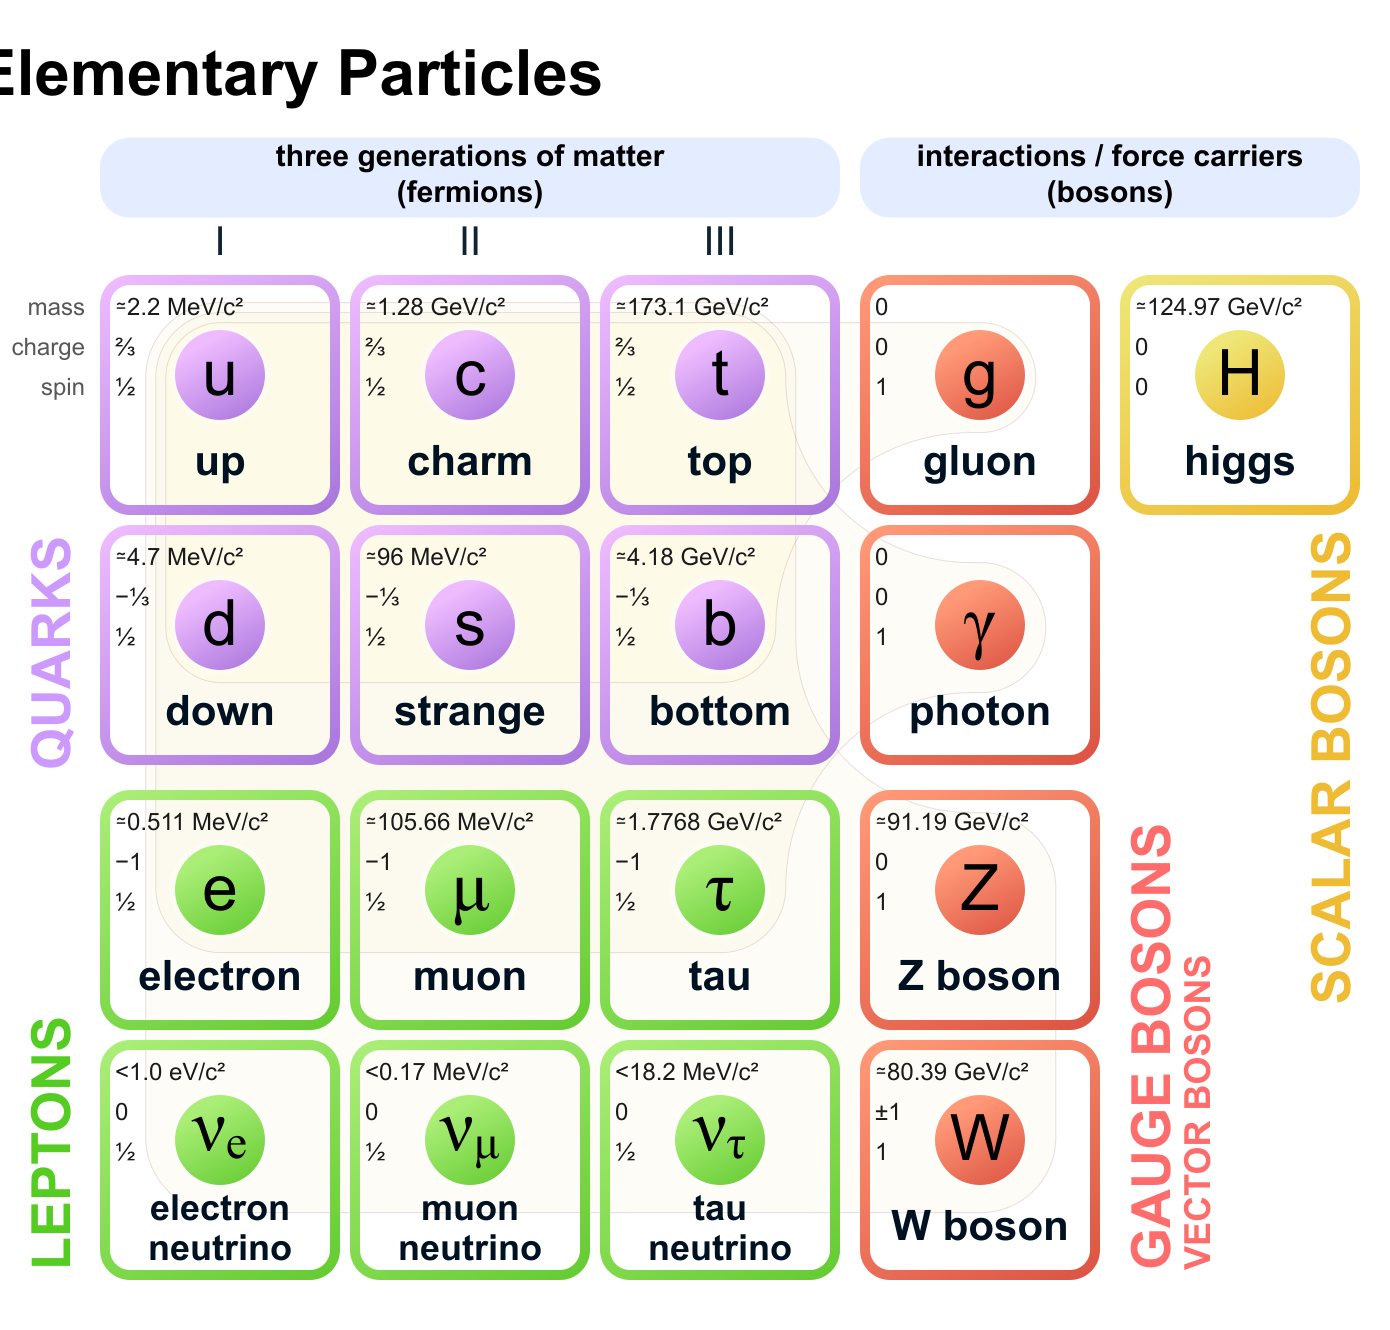
\includegraphics[width=0.7\textwidth]{figures/Fig14}
	\caption{The particle content of the Standard Model.}
	\label{Fig14}
\end{figure}
\section{Z boson production at the LHC}\label{chap2sec0}
Since the discovery of the Z boson at the UA1 and UA2 experiments \cite{Arnison:1983rp,Arnison:1983mk,Banner:1983jy,Bagnaia:1983zx}, it has been the subject of multiple measurements in proton-proton and electron-positron colliders. The Z boson mass $m_Z=91.1875\pm0.0021$ GeV and its decay width $\Gamma_Z=2.4952\pm0.0023$ GeV have been measured to outstanding precision \cite{ALEPH:2005ab}. The braching ratios of the Z boson are well known; they are presented in Table \ref{Table0}.
\begin{table}[]
	\centering
	\begin{tabular}{cc}
		\hline
		\multicolumn{1}{|c|}{Decay mode} & \multicolumn{1}{c|}{Branching fraction (\%)} \\ \hline
		$e^+e^-$                         & $3.363\pm0.004$                              \\
		$\mu^+\mu^-$                     & $3.366\pm0.007$                              \\
		$\tau^+\tau^-$                   & $3.370\pm0.008$                              \\
		Invisible                        & $20.00\pm0.06$                               \\
		Hadrons                          & $69.91\pm0.06$                               \\ \hline
	\end{tabular}
	\caption{Z boson branching fractions.}
	\label{Table0}
\end{table}
In contrast to electron-positron colliders, the momentum of partons in proton-proton collisions is not precisely known. Thus, parton density functions (PDFs) are used to describe the proton structure in a phenomenological way. These functions are written as $f_{a/A}(x,Q^2)$ and represent the probability density for a parton $a$ to have a fraction $x=\frac{p_a}{p_A}$ of the proton momentum $p_A$. $Q$ is the energy scale of the scattering process. In this case, the cross section of two protons going to a final state $n$ will be
\begin{equation}
	\sigma_{p_Ap_B\to n}=\sum_{q}\int dz_adx_b f_{a/A}(x_a,Q^2) f_{b/B}(x_b,Q^2)\times [\sigma_0+\alpha_s\sigma_1+\dots]_{ab\to n}.
\end{equation}
The sum is made over all the partons. $\sigma_0$ is the tree level parton-parton cross section and $\sigma_1$ are the QCD corrections to first order. A diagram of the production of the Z boson in proton-proton collisions is shown in Fig.\ref{Fig15}. 
\begin{figure}[h]
	\centering
	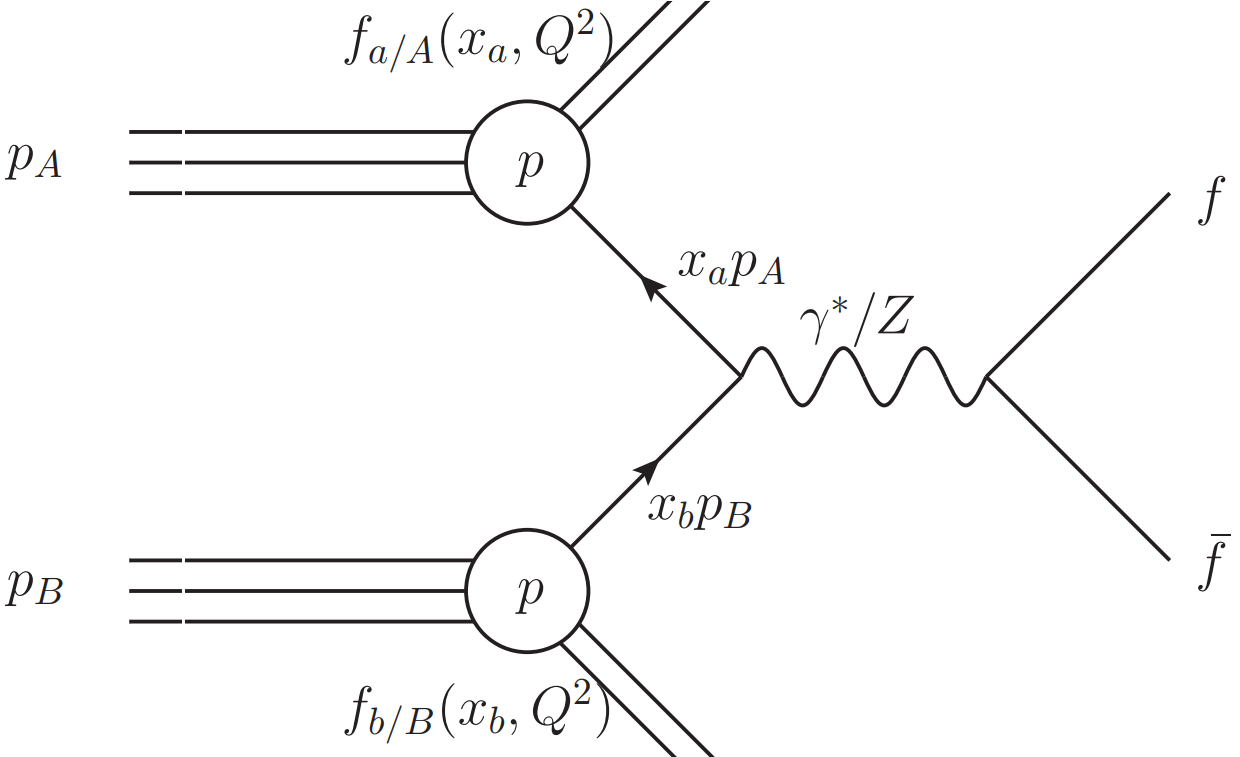
\includegraphics[width=0.6\textwidth]{figures/Fig15}
	\caption{Illustration of the production of a Z boson in pp collisions via quark-antiquark annihilation.}
	\label{Fig15}
\end{figure}
The main process contributing to Z boson production is the Drell-Yan process, where a quark-antiquark ($q\bar{q}$) pair annihilate, produce a Z boson and it subsequently decays into a pair of fermions. In this case, the transverse momentum ($\pt$) of the Z boson comes from the intrinsic $\pt$ of the partons. Nevertheless, this has been experimentally determined with a value of $<k_T>=0.76$ GeV \cite{Ellis:1991qj} and is not large enough to explain the measured Z boson $\pt$ distribution that peaks at a few GeV and has a tail that extends at values $\pt\gg m_Z$ \cite{Abbott:1999yd,Affolder:1999jh}.

To explain this kinematic feature we have to look at the other ways the Z boson can be produced in $pp$ collisions. First quark-gluon ($qg$) scattering, where the Z boson recoils against the quark radiated in the final state, this process is illustrated in Fig.\ref{Fig16a}. In the other hand, we could also have a gluon being radiated before $q\bar{q}$ annihilation takes place, having the Z boson recoiling against what is called \textit{initial state radiation} (ISR), as is shown in Fig.\ref{Fig16b}. Partons generated in $qg$ scattering and FSR pair with other quarks and gluons to form showers of \textit{hadrons} (this showers are usually called jets) that are subsequently detected as energy deposits in the calorimeters of the particle detectors. 
\begin{figure}[ht]
	\centering
	\subfloat[]{\label{Fig16a}{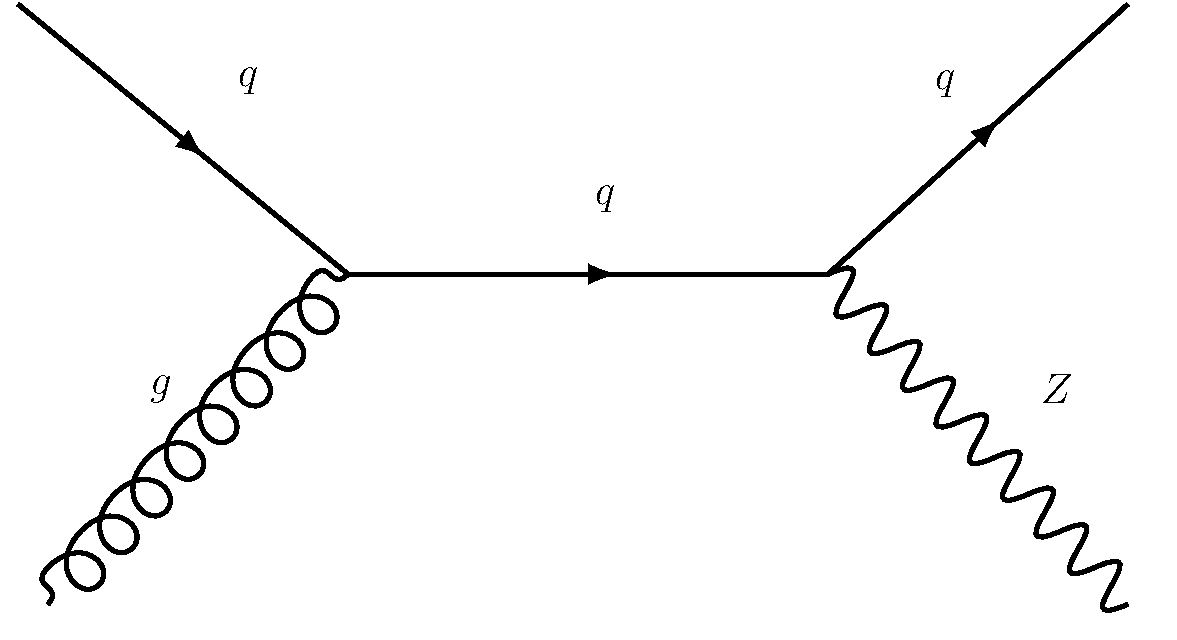
\includegraphics[width=0.50\textwidth]{figures/Fig16a}}}\hfill
	\subfloat[]{\label{Fig16b}{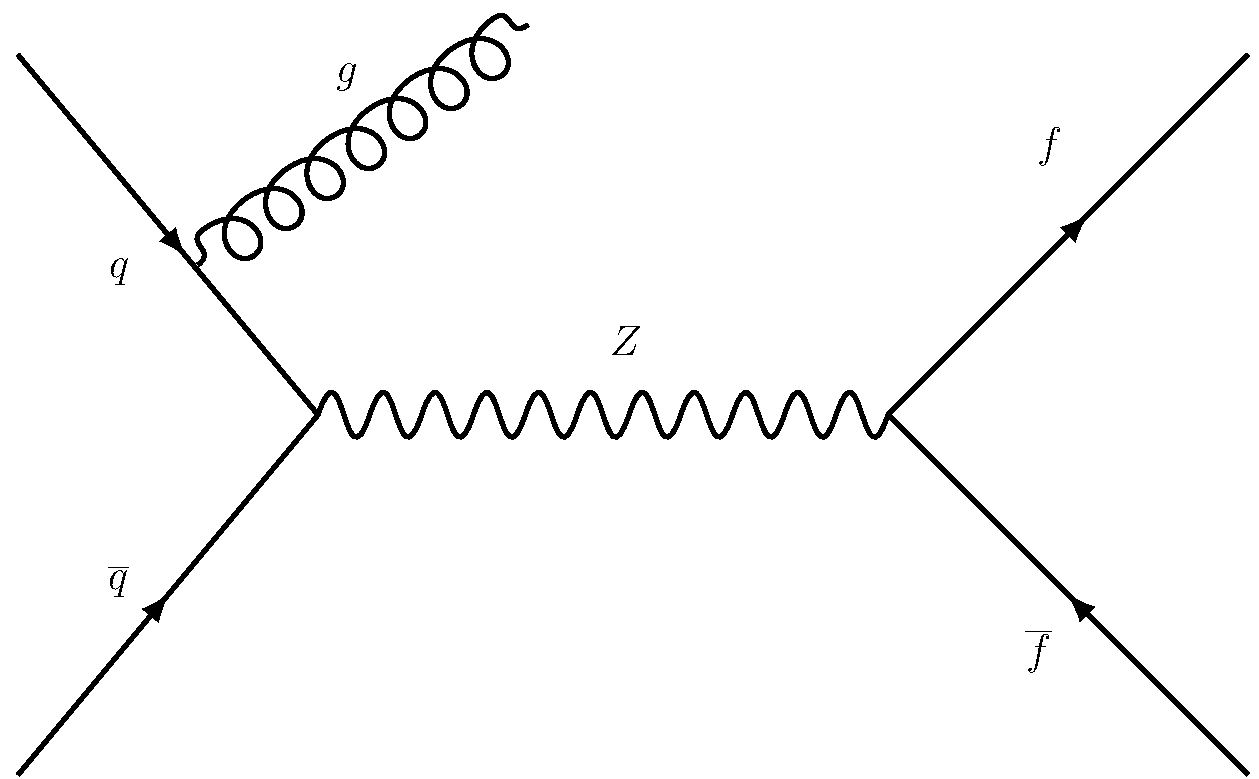
\includegraphics[width=0.50\textwidth]{figures/Fig16b}}}
	\caption{$qg$ Z boson production with FSR (a) and $q\bar{q}$ annihilation with gluon ISR (b).}
	\label{Fig16}
\end{figure}
\section{The Tau Lepton}\label{chap2sec1}
The tau, is a spin-$\frac{1}{2}$ charged particle that belongs to the family of leptons. The first hints of the tau existence came from experiments conducted at the Stanford Linear Accelerator Center and Lawrence Berkeley National Laboratory \cite{PhysRevLett.35.1489}. They discovered 64 events of the form:
\begin{equation}
	e^+ + e^- \to e^\pm + \mu^\mp + \geq \text{2 undetected particles},
\end{equation}
for which there was no conventional explanation at the time. Later on, it was discovered that these events came from the production of a pair of new particles, two taus that subsequently decayed into one electron, a muon and four neutrinos. Events like,
\begin{equation}
e^+ + e^- \to \tau^+ \tau^- \to e^\pm + \mu^\mp + 4\nu,
\end{equation}	
were later explored to derive tau mass and spin, confirming the existence of a third generation of leptons. 

The tau has a mass of $1776.86 \pm 0.12$ MeV \cite{PhysRevD.98.030001}, which allows it to decay not only into the other lighter lepton generations (\textit{leptonic tau decays}), as shown on Fig.\ref{Fig1}  , but into hadrons. As we said on section \ref{chap2sec0} hadrons are particles made of quarks. All the decay channels of the tau containing hadrons in the final state are called \textit{hadronic tau decays}. Strictly speaking this is a semi-hadronic decay mode because of the presence of the neutrino. Nonetheless, from now on we will refer to these processes with the commonly used term \textit{hadronic tau decays}. An example of this decay mode is shown in Fig.\ref{Fig2}.
\begin{figure}[h]
	\centering
	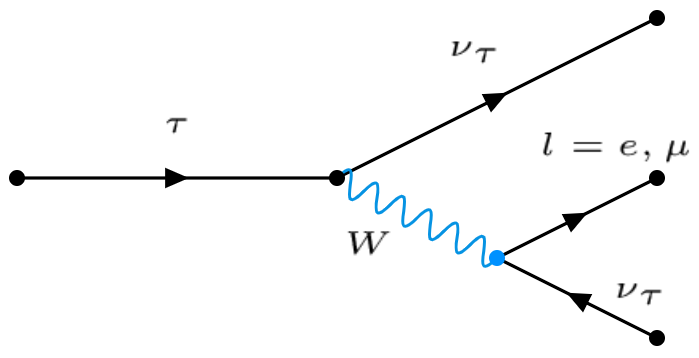
\includegraphics[width=0.6\textwidth]{figures/Fig1}
	\caption{Tau leptonic decay mode. Tau lepton is kinematically allowed to decay into muons or electrons, note that in this decay mode two neutrinos of different flavour are produced.}
	\label{Fig1}
\end{figure}
\begin{figure}[h]
	\centering
	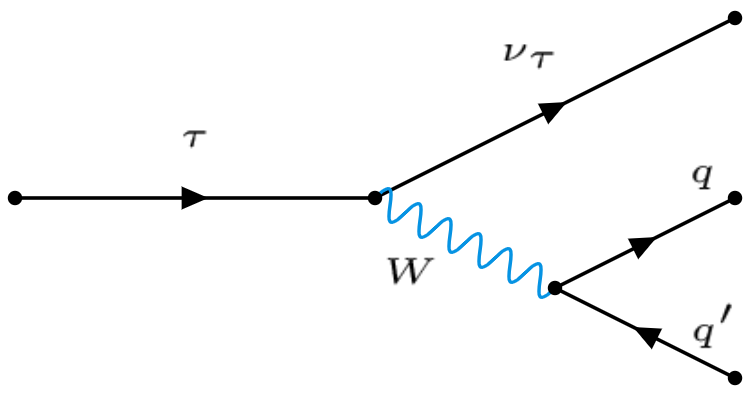
\includegraphics[width=0.6\textwidth]{figures/Fig2}
	\caption{Tau hadronic decay mode. The tau lepton is kinematically allowed only to decay into hadrons containing up, down and strange quarks. This results on final states containing multiple pions or kaons \cite{Davier_2006}.}
	\label{Fig2}
\end{figure}
Naively, if we were to estimate the branching fraction for hadronic and leptonic tau decay modes, defined as
\begin{equation}
	\beta(\tau\to X\nu_\tau)=\frac{\Gamma(\tau\to X\nu_\tau)}{\Gamma_{\text{tot}}}.
\end{equation}
Where $X$ could be any number of leptons or hadrons and $\Gamma_{\text{tot}}$ is the total decay width for the tau. We could argue that the contribution from the hadronic decays triples the contribution for one of the leptonic modes. This is because in any hadronic decay, we would have to count 3 different diagrams, like the one in Fig.\ref{Fig2} because of the three colour possibility for the quarks.

Thus, 
\begin{align}
\beta(\tau\to l\nu_l\nu_\tau)\approx 20\%& \hspace{1cm}l=e,\mu;
\\
\beta(\tau\to X\nu_\tau)\approx 60\%& \hspace{1cm} X=\text{hadrons+neutrinos}.
\end{align}
In fact, this naive estimation is not bad. Actual values for the leptonic branching ratios are \cite{PhysRevD.98.030001}:
\begin{align}
\beta(\tau\to e\nu_e\nu_\tau)&=17.82\pm 0.04\%
\label{eq6}
\\
\beta(\tau\to \mu\nu_\mu\nu_\tau)&=17.39\pm 0.04\%.
\end{align}
The reason of the difference in the estimation is that in the case of the W decaying to quark pairs, there is a non-negligible contribution that comes of the mixing from quark pairs of different generations. In particular, in the tau decay we are talking about the contribution from up-strange quark couplings. This is the Cabibbo suppressed amplitude and it is proportional to the $V_{us}$ component of the CKM matrix \cite{Davier:2005xq}. The small difference between the leptonic branching fractions is due to the mass difference between the muon and the electron.

On the other hand, the hadronic decays of the tau are more varied and can contain many more particles in the final states. The vast majority of hadronic tau decays have charged or neutral pions in the final states, but more exotic decays including kaons also happen. Branching fractions for the most important tau hadronic decays are showed in Table \ref{Table1}.
\begin{table}[]
	\centering
\begin{tabular}{|c|c|}
	\hline
	Decay mode                     & Branching fraction \\ \hline
	$\pi^\pm \nu_\tau$             & 11.1 \%            \\ \hline
	$\pi^\pm \pi^0 \nu_\tau$       & 25.4\%             \\ \hline
	$\pi^\pm \geq 2\pi^0 \nu_\tau$ & 9.1\%               \\ \hline
	$3\pi^\pm \nu_\tau$            & 9.1\%               \\ \hline
	$3\pi^\pm \geq 1\pi^0 \nu_\tau$& 4.6\%               \\ \hline
	others						   & 5.5\%               \\ \hline
\end{tabular}
	\caption{Branching fractions for hadronic tau decay modes \cite{PhysRevD.98.030001}.}
	\label{Table1}
\end{table}
\section{Lepton Universality}\label{chap2sec2}
The SM predicts that all charged leptons $(e,\mu,\tau)$ interact via the electromagnetic and weak forces and explains that these interactions can be seen as the interchange of \textit{vector bosons}, the photon $(\gamma)$ and the W and Z bosons respectively. Specifically, in the SM the form of the interaction does not depend on the lepton generation. This feature of the SM is called \textit{lepton universality} and it can be understood as that physical processes for electrons, muons and taus are almost identical copies of each other (although some small discrepancies arise from the fact that lepton masses). 

For instance, tau leptonic decay widths present a great opportunity to test lepton universality hypothesis. If we start considering muon decay, at low energies we can consider this process to be a point like interaction well described by Fermi theory \cite{FermiTheory}. In this case, if we approximate the electron and neutrinos as being massless particles, a dimensionally correct expression for the width is of the form
\begin{equation}
	\Gamma(\mu\to e+\nu_e +\nu_\mu)=KG_{F}^{2}m_{\mu}^{5},
\end{equation} 
where $G_F=1.1666\times 10^{-5} \text{ GeV}^{-2}$ is the Fermi coupling constant and $K$ is a constant that depends on the form of the interaction. If we assume that lepton universality holds, the respective widths for the tau leptonic decay modes, will have the form
\begin{align}
\Gamma(\tau\to e+\nu_e +\nu_\tau)&=KG_{F}^{2}m_{\tau}^{5},
\\
\Gamma(\tau\to \mu+\nu_\mu +\nu_\tau)&=\Gamma(\tau\to e+\nu_e +\nu_\tau),
\end{align}  
which explains why to a good approximation leptonic branching fractions for tau decay are equal. Moreover, we can obtain a relation between tau and muon lifetimes. We know that,
\begin{equation}
	\tau_l=\frac{1}{\Gamma_\text{Tot}}=\frac{\beta(l\to e\nu_e \nu_l)}{\Gamma(l\to e\nu_e \nu_l)},
	\label{eq11}
\end{equation}
also that $\beta(\mu\to e\nu_e \nu_\mu)=1$ and taking into account eq.(\ref{eq6}) we can take the ratio between eq.(\ref{eq11}) for $l=\tau ,\mu$ to obtain
\begin{equation}
\frac{\tau_\tau}{\tau_\mu}=\frac{\beta(\tau\to e\nu_e \nu_\tau)}{\beta(\mu\to e\nu_e \nu_\mu)}\left(\frac{m_\mu}{m_\tau}\right)^5=(1.328\pm 0.004)\times 10^{-7}.
\end{equation}
This is consistent with the experimental lifetimes ratio of $(1.3227\pm 0.0005)\times10^{-7}$ \cite{Martin:1992rg}. This agreement on lifetimes that differ on 7 orders of magnitude is a good proof that lepton universality holds on W decays at the tau mass scale.

Very precise tests of LU have been done by $e^-e^+$ colliders (LEP1, SLC and LEP2). Measurements of the ratios between the leptonic decay widths of the Z boson have been performed and are consistent with the SM \cite{ALEPH:2005ab}:
\begin{align}
	\frac{\Gamma(Z\to\mu^+\mu^-)}{\Gamma(Z\to e^+e^-)}=1.0009\pm 0.0028,
	\\
	\frac{\Gamma(Z\to\tau^+\tau^-)}{\Gamma(Z\to e^+e^-)}=1.0019\pm 0.0032.
\end{align}
LU has also been tested in W boson decays. A combination of measurements made by different experiments of the branching fractions between the first two families of leptons are consistent with SM predictions \cite{Pich:2013lsa}:
\begin{equation}
\frac{\beta(W^-\to e^-\bar{\nu_e})}{\beta(W-\to \mu^-\bar{\nu_\mu})}=1.004\pm 0.008.
\end{equation}
But measurements including the third lepton family, apart from being less precise due to the more challenging reconstruction of the $\tau$ lepton final states are in tension with SM \cite{Schael:2013ita}:
\begin{align}
\frac{\Gamma(W^-\to\tau^-\bar{\nu_\tau})}{\Gamma(W^-\to e^-\bar{\nu_e})}=1.063\pm 0.027,
\\
\frac{\Gamma(W^-\to\tau^-\bar{\nu_\tau})}{\Gamma(W^-\to \mu^-\bar{\nu_\mu})}=1.070\pm 0.026.
\end{align}
These results show that LU between the two first lepton family holds with a precision of 0.3\% and 0.8\% in Z and W decays respectively. Constraints between the third and the other two generations of leptons are of similar precision on Z boson decays (0.3\%), but ten times worse for W boson decays (3\%) and somewhat in tension with SM prediction. An example of this is a measurement exhibiting a tension of 2.6 $\sigma$ from the SM expectation \cite{Schael:2013ita}:
\begin{equation}
	\frac{2\Gamma(W^-\to\tau^-\bar{\nu_\tau})}{\Gamma(W^-\to e^-\bar{\nu_e})+\Gamma(W^-\to \mu^-\bar{\nu_\mu})}=1.066\pm 0.025.
\end{equation}  


Furthermore, measurements from LHCb, BaBar and Belle experiments have shown consistent deviations from the SM predictions \cite{Ciezarek_2017}. These experiments have independently measured a deviation on $\bar{B}$ meson semi-leptonic branching ratios, specifically:
\begin{align}
	R_D&=\frac{\beta(\bar{B}\to D\tau^-\bar{\nu}_\tau)}{\beta(\bar{B}\to De^-\bar{\nu}_e)}
	\\
	R_{D^\star}&=\frac{\beta(\bar{B}\to D^\star\tau^-\bar{\nu}_\tau)}{\beta(\bar{B}\to D^\star e^-\bar{\nu}_e)}.
\end{align}
The combined results for the different experiments are shown in Fig.\ref{Fig3}. These measurements represent a 3.08 $\sigma$
 deviation from the SM predictions, but even though they represent a hint of new physics, these results have to be taken with care since at this point it could be that statistical deviations are larger than expected. In this matters, future analysis from experiments like LHCb and Belle II with larger available datasets will be very important to untangle this situation.
 \begin{figure}[h]
 	\centering
 	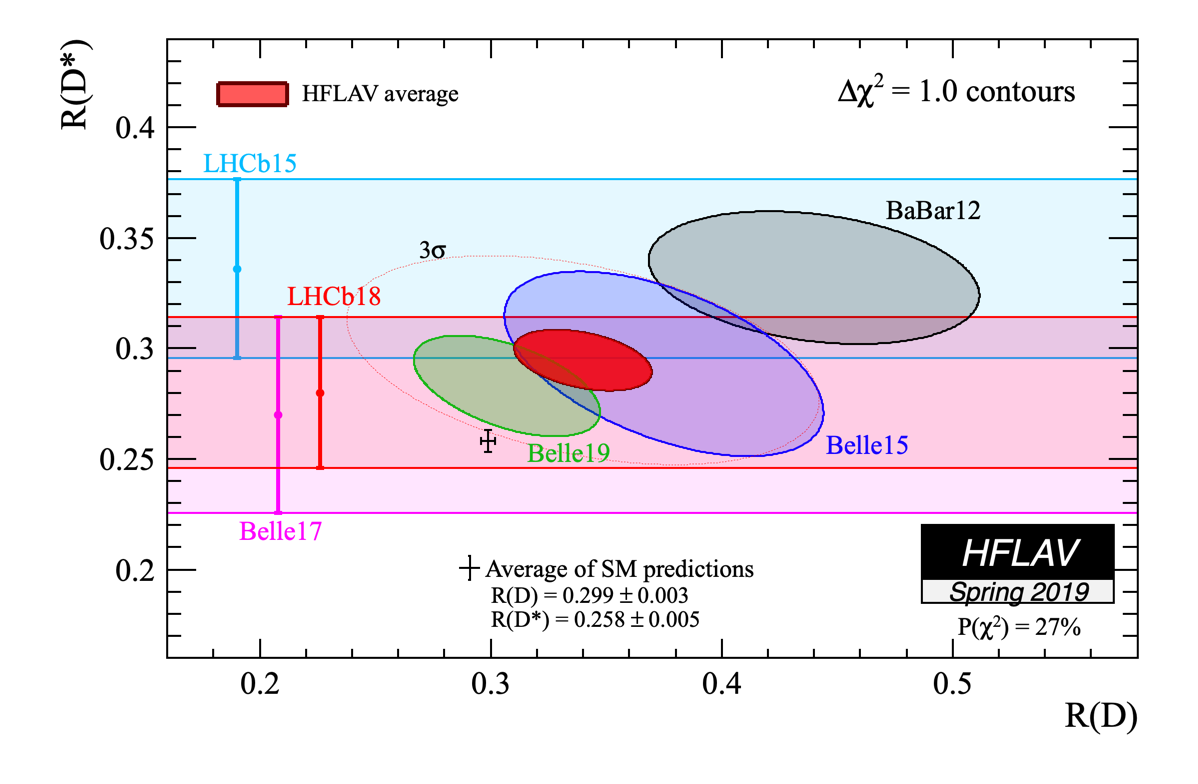
\includegraphics[width=0.7\textwidth]{figures/Fig3}
 	\caption{Combined results from BABAR, Belle and LHCb with 1-$\sigma$ contour. The average calculated by the Heavy Flavour Averaging Group \cite{HFAG}  is compared with the SM predictions.}
 	\label{Fig3}
 \end{figure}